\documentclass[10pt,a4paper]{article}
\usepackage[utf8]{inputenc}
\usepackage{titlesec}
\usepackage{amsfonts}
\usepackage{graphicx}
\usepackage{hyperref}
\usepackage{amsmath}
\usepackage{amssymb}
\usepackage{multicol}
\usepackage{array}
\usepackage{color}
\usepackage{float}
\usepackage[left=2.50cm, right=2.00cm, top=2.50cm, bottom=2.50cm]{geometry}
\usepackage[txtcentered=true, height=40pt, width=70pt]{thumbs}
\usepackage[german]{babel}
\usepackage{subfigure}
\usepackage[justification=centering]{caption}
\author{Florian Euchner, Stefan Köbel, Chong Shen, Jan Frederik Dick}

\newcommand{\fancythumb}[2]{
	\addthumb{#1}{\large\sffamily\textbf{\space\space#1\vspace{5pt}}}{white}{#2}
}

\newcommand{\fancyformula}[2]{
	\small
	\raggedright\sffamily\textbf{#1}
	#2
}

\pagenumbering{arabic}
\titleformat*{\section}{\sffamily\huge\bfseries}
\titleformat*{\subsection}{\sffamily\Large\bfseries}
\titleformat*{\subsubsection}{\sffamily\large\bfseries}

\begin{document}
\section*{Signale und Systeme}
\fancythumb{S\&S}{teal}
\subsection*{Signal}
Ein Signal ist eine \textbf{Funktion} $x(t)$. Sie liefert für jedes Funktionsargument $t$ einen Funktionswert $x(t)$.
\subsection*{Klassifikation von Signalen}
\begin{itemize}
	\item \textbf{gerade/ungerade}: $x(t)=x_g(t)+x_u(t)$, wobei $x_g(-t)=x_g(t)$ und $x_u(-t)=-x_u(t)$, $x_u(0)=0$
	\item \textbf{reell/imaginär/komplex}: $x(t)=x_r(t)+jx_i(t)$ und $x^*(t)=x_r(t)-jx_i(t)$, wobei $x^*(t)$ komplex konjugiert zu $x(t)$, Realteil: $x_r(t)=\dfrac{1}{2}(x(t)+x^*(t))$ und Imaginärteil: $x_i(t)=\dfrac{1}{2j}(x(t)-x^*(t))$ 
	\item \textbf{periodisch}: es existiert $T$, sodass $x(t+T)=x(t)$ für alle $t$; Kleinstes $T$ heißt dann Periode
	\item \textbf{einkanalig}: ein Funktionswert, z.B. $x(t)$
	\item \textbf{mehrkanalig}: mehrere Funktionswerte, z.B.
	$\begin{bmatrix}
		x_1(t) \\ 
		x_2(t)
	\end{bmatrix}$
	\item \textbf{eindimensional}: ein Funktionsargument, z.B. $x(t)$
	\item \textbf{mehrdimensional}:mehrere Funktionsargumente, z.B. $x(t,x,y)$
	\item \textbf{zeitkontinuierlich}: zeitkontinuierliches Funktionsargument, $x(t)$ mit $t \in \mathbb R$
	\item \textbf{zeitdiskret}: zeitdiskretes Funktionsargument, $x(n)$ mit $n \in \mathbb Z$
	\item \textbf{wertkontinuierlich}: kontinuierlicher Funktionswert
	\item \textbf{wertdiskret}: diskreter Funktionswert
	\item \textbf{analog}: zeitkontinuierliche und wertkontinuierlich
	\item \textbf{digital}: zeitdiskret und wertdiskret
\end{itemize}
\subsection*{Zeitkontinuierliche Signale}
\begin{itemize}
	\item Sprungfunktion
	\item Vorzeichenfunktion
	\item Rechteckfunktion
	\item Reelles oder komplexes Sinussignal
	\item Exponentialsignal
	\item verschobenes Rechteck
	\item Dreieck
\end{itemize}
\subsection*{Zeitdiskrete Signale}
\begin{itemize}
	\item Sprungfunktion
	\item Vorzeichenfunktion
	\item Rechteckfunktion
	\item Reelles oder komplexes Sinussignal
	\item Exponentialsignal
\end{itemize}
\subsection*{System}
	Das System hat einen \textbf{Operator}, der eine Funktion auf eine andere Funktion abbildet. Ein System heißt \textbf{zeitkontinuierlich, zeitdiskret, analog, digital}, wenn alle beteiligten Signale so heißen.
\subsection*{Klassifikation von Systemen}
\begin{itemize}
	\item Gedächtnis
	\item Kausalität
	\item Zeitvarianz
	\item Linearität
	\item BIBO-Stabilität
\end{itemize}
\subsection*{Parallel- und Kettenschaltung von Systemen}
\begin{itemize}
	\item \textbf{Parallelschaltung} $y(t)=T_1(x(t))+T_2(x(t))+...+T_N(x(t))$
	\item \textbf{Kettenschaltung} 	$y(t)=T_N(...T_2(T_1(x(t)))...)$
\end{itemize}

\newpage


\section*{Zeitkontinuierliche LTI-Systeme im Zeitbereich}
\fancythumb{ZK-t}{red}
\subsection*{Impulsantwort und Sprungantwort}
\subsection*{Faltung}
\subsubsection*{Grafische Faltung}
\begin{figure}[H]
	\centering
	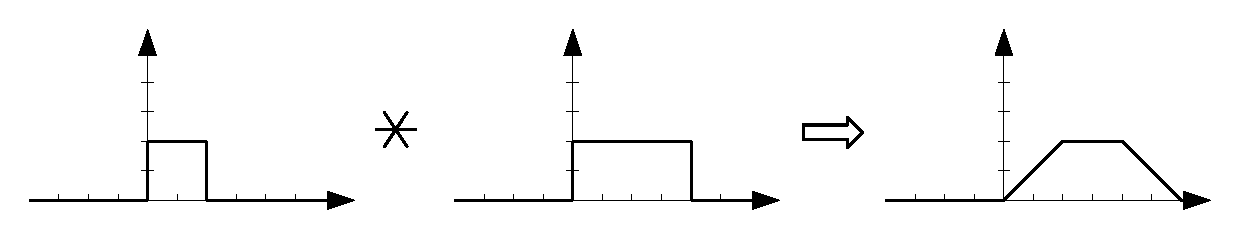
\includegraphics[width=0.75\textwidth]{img/faltung1.pdf}
	\caption*{Faltung zweier Rechtecksignale}
\end{figure}
\begin{figure}[H]
	\centering
	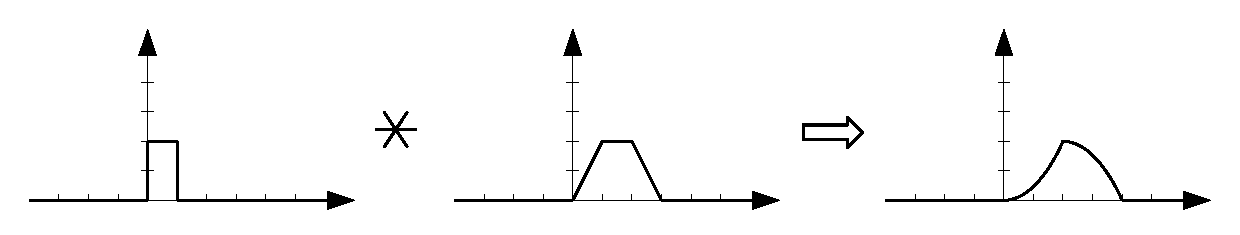
\includegraphics[width=0.75\textwidth]{img/faltung2.pdf}
	\caption*{Faltung eines Rechtecks mit einem Signal mit zwei linearen Flanken}
\end{figure}
\begin{figure}[H]
	\centering
	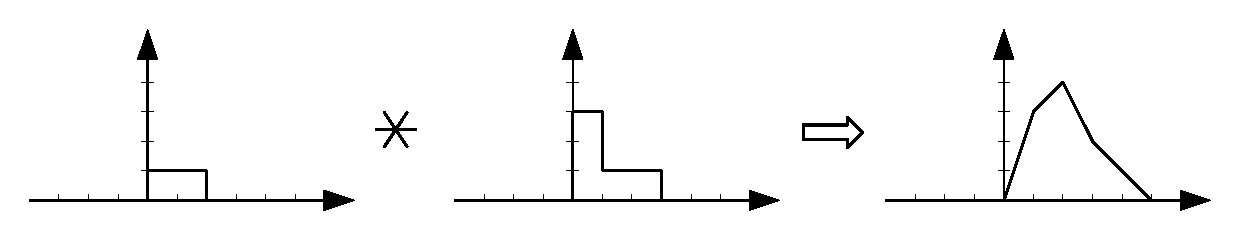
\includegraphics[width=0.75\textwidth]{img/faltung3.pdf}
	\caption*{Faltung verschieden hoher Rechtecksignale}
\end{figure}
\subsubsection*{Analytische Faltung}
\paragraph*{Definition}
\[ (f \ast g)(t)=\int_\mathbb{R}f(\tau)\cdot g(t-\tau) d\tau \]
Das Ausgangssignal $y(t)$ eines Systems ist das Eingangssignal $x(t)$ mit der Impulsantwort $h(t)$ gefaltet.
\[ y(t) = (x \ast h)(t)=\int_\mathbb{R}x(\tau)\cdot h(t-\tau) d\tau\]
\subsection*{Überprüfung von Eigenschaften von LTI-Systemen mit Impulsantwort}
\newpage


\section*{Zeitdiskrete LTI-Systeme im Zeitbereich}
\fancythumb{ZD-t}{magenta}
\subsection*{Lineare Differenzengleichungen mit konstanten Koeffizienten}
\begin{tabular}{r p{12cm}}
	\textbf{DGL} & $\alpha(D) ~ y(n) = \beta(D) ~ x(n)$, wobei $D^k(y) = y(n-k)$ und $\alpha$, $\beta$ Polynome vom Grad N bzw. M \\
	\textbf{Eingangssignal} & $x(n) = u(n) ~ A ~ q^n$ \\
	\textbf{Anfangswerte} & $y(-1)$, …, $y(-N)$ und (wenn nicht aus $x(n)$ ersichtlich) $x(-1)$, …, $x(-M)$ \\
	\textbf{Lösung} & Funktion $y(n)$ für $n \geq 0$, die DGL für Eingangssignal erfüllt. $y(n)$ muss nicht die Anfangsbedingungen erfüllen, da $n \geq 0$
\end{tabular}

\subsubsection*{Homogene Lösung $y_h$}
Bestimme $y_h(n)$, sodass $\alpha(D) ~ y_h(n) = 0 ~ \forall n \in \mathbb Z$. Bestimme alle $\tilde N$ verschiedene Nullstellen $z_1$, …, $z_{\tilde N}$ der Gleichung $\alpha(z^{-1}) = 0$ nach durchmultiplizieren mit $z^N$.

\paragraph{Nullstellen verschieden:} Jede Nullstelle ist einfach $\Leftrightarrow \tilde N = N$
\[
	y_h(n) = c_1 ~ z_1^n + … + c_N ~ z_N^n
\]

\paragraph{Mehrfache Nullstellen:} $z_1$ ist $k$-fache Nullstelle $\implies \tilde N = N - k < N$
\[
	y_h(n) = \left(c_{1,1} + c_{1,2} ~ n + … + c_{1,k} ~ n^{k-1}\right) ~ z_1^n + c_2 ~ z_2^n + … + c_{\tilde N} ~ z_{\tilde N}^n
\]

\subsubsection*{Partikuläre Lösung $y_p$}
Bestimme ein $y_p(n)$ so, dass $\alpha(D) ~ y_p(n) = \beta(D) ~ x(n) ~ \forall n \geq 0$ für ein spezifisches $x(n) = u(n) ~ A ~ q^n, n \geq 0$.

\paragraph{q keine Nullstelle von $\alpha \Leftrightarrow q \neq z_i ~ \forall i$}
\[
	y_p(n) = A ~ \frac{\beta(q^{-1})}{\alpha(q^{-1})} ~ q^n
\]
\paragraph{q ist k-fache Nullstelle von $\alpha \Leftrightarrow \exists i: ~ q = z_i$} Mit $\alpha^{(k)}(D)$ ist k-te Ableitung von $\alpha(D)$:
\[
	y_p(n) = A ~ \frac{\beta(q^{-1})}{\alpha^{(k)}(q^{-1})} (-q ~ n)^k ~ q^n
\]

\subsubsection*{Allgemeine Lösung $y$ und Lösung mit Anfangswerten}
\[
	y(n) = y_h(n) + y_p(n)
\]
Um die Anfangswerte zu berücksichtigen, müssen Koeffizienten $c_1, …, c_N$ bzw. $c_{1,0}, …, c_{1,k}, …, c_{\tilde N}$ bestimmt werden. Setze dazu Werte von $x(n)$ und $y(n)$ in Abhängigkeit der Koeffizienten in die DGL für $n = 0, …, N - 1$ ein und Löse LGS.

\vspace{.5em}
\raggedright
\textbf{Warnung:} \textit{Nicht} die Koeffizienten durch Lösen von $y(-1) = y(n)$ für $n = -1$ etc. bestimmen - das wird falsch, denn $y(n)$ ist für $n < 0$ keine Lösung, da $y_p$ dann keine Lösung!

\subsubsection*{Impulsantwort $h$}
Für Anfangsbedingungen gilt $y(-1) = … = y(-N) = 0$.
\paragraph{Für $N > M$:} Es ist klar, dass $\alpha(D) ~ y_h(n) = 0 ~ \forall n \in \mathbb Z$ für beliebige Koeffizienten $c$. Nun wird das System mit der Impulsfunktion 
\[
	\delta(n) =
	\begin{cases}
		1 & \textnormal{für } n = 0 \\
		0 & \textnormal{sonst}
	\end{cases}
\]
angeregt. Für $n > M$ ist die Differenzengleichung also homogen, da auf der rechten Seite $x(n) = \delta(n)$ höchstens in der $M$-ten Verzögerung $D^M ~ x(n) = \delta(n - M) = 0$ steht.

\vspace{.5em}
Ansatz: Impulsantwort $h(n) = y(n) = u(n) ~ y_h(n)$ stimmt schon für $n > M$, bestimmte Koeffizienten so, dass $h(n)$ auch für $n = 0, …, M$ passt. Berechne LGS durch Einsetzen von $y(n)$, $x(n) = \delta(n)$ in DGL für $n = 0, …, N - 1$ mit $N$ Gleichungen und den $N$ unbekannten Koeffizienten $c$.

\[
	h(n) = u(n) ~ y_h(n) ~~ \textnormal{…mit den durch LGS bestimmten Koeffizienten $c$}
\]

\paragraph{Sonst:} Setze Eingangssignal $x(n) = u(n) ~ A ~ q^n$ zu $A = q = 1$, sodass $x(n) = u(n)$. Bestimme allgemeine Lösung der DGL mit diesem Eingangssignal, Lösung ist Sprungantwort $a(n) = y(n)$.

\vspace{.5em}
Da gilt $\delta(n) = u(n) - u(n - 1)$ folgt aus Linearität mit Systemoperator $T$ und $T(\delta(n)) = T(u(n) - u(n - 1))$:
\[
	h(n) = a(n) - a(n-1)
\]

\newpage


\section*{Zeitkontinuierliche LTI-Systeme im Frequenzbereich}
\fancythumb{ZK-f}{blue}
\subsection*{Fourierreihe}
\subsubsection*{Definition}
\[
	x(t) = \sum_{k=-\infty}^\infty c_k ~ e^{jk\Omega t} = a_0 + \sum_{k=1}^\infty \left( a_k ~ \cos(k \Omega t) + b_k ~ \sin(k \Omega t) \right)
\]

\begin{centering}
\begin{tabular}{ >{\centering\arraybackslash} m{7cm} >{\centering\arraybackslash} m{1cm} >{\centering\arraybackslash} m{7cm} }

\[
	c_k = \frac{1}{T} ~ \int_T x(t) ~ e^{-jk\Omega t} \mathrm dt
\] & \textit{\sffamily oder} & {
\[
	a_0 = \frac{1}{T} \int_T x(t) \mathrm dt
\]
\[
	a_k = \frac{2}{T} \int_T x(t) ~ \cos(k\Omega t) \mathrm dt, ~ k \in \mathbb Z
\]
\[
	b_k = \frac{2}{T} \int_T x(t) ~ \sin(k\Omega t) \mathrm dt, ~ k \in \mathbb Z
\]
}\\
\end{tabular}
\end{centering}

\newpage
\section*{Eigenschaften der Fouriertransformation}
\begin{multicols}{2}
	
\fancyformula{Definition}{
	\[ X(j\Omega)=\int_{-\infty}^{\infty}x(t)e^{-j\Omega t}dt \]
}
\end{multicols}

\newpage
\section*{Zeitdiskrete LTI-Systeme im Frequenzbereich}
\fancythumb{ZD-f}{violet}

\newpage
\section*{Analyse von Signalen und LTI-Systemen in der komplexen Ebene}
\fancythumb{$\mathbb{C}$}{olive}

\newpage
\section*{Allgemeinere Signale und Systeme}
\fancythumb{Allg. S\&S}{black}
\end{document}
